\documentclass[aip,jcp,reprint,amsmath,amssymb]{revtex4-2}

\usepackage[utf8]{inputenc}
\usepackage[T1]{fontenc}
\usepackage{graphicx}
\usepackage{booktabs}
\usepackage[version=4]{mhchem}
\usepackage{siunitx}
\usepackage{xspace}
\usepackage{url}

\graphicspath{{../figures/}{figures/}}

\newcommand{\waterair}{water--air\xspace}
\newcommand{\sfg}{SFG\xspace}
\newcommand{\chis}{\ensuremath{\chi^{(2)}}\xspace}
\newcommand{\imchi}{\ensuremath{\mathrm{Im}\,\chi^{(2)}}\xspace}

\begin{document}

\title{The Silica/Water Interface Revisited: Elucidating Interfacial Water Structure with an SFG Rosetta Stone}

\author{Jen{\'e}e D. Cyran}
\affiliation{Department of Chemistry and Biochemistry, Boise State University, Boise, Idaho 83725, United States}

\author{Thomas D. K{\"u}hne}
\email{tkuehne@cp2k.org}
\affiliation{Center for Advanced Systems Understanding (CASUS), 02826 G{\"o}rlitz, Germany}
\affiliation{Helmholtz-Zentrum Dresden-Rossendorf, 01328 Dresden, Germany}
\affiliation{Institute of Artificial Intelligence, Technische Universit{\"a}t Dresden, 01069 Dresden, Germany}

\date{\today}

\begin{abstract}
Phase-resolved vibrational sum-frequency generation (SFG) reports on interfacial water with orientational sensitivity, but converting an OH-stretch spectrum into a molecular structure remains an underdetermined inverse problem. We analyze the buried silica/water response trace of Cyran \textit{et al.} with species-resolved water--air SFG fingerprints as a structural Rosetta stone. The analysis is performed in the silica-side viewing convention, where positive \imchi corresponds to OH/H orientation toward the silica window. The analysis window is selected from the experimental trace itself: the \SIrange{3200}{3300}{cm^{-1}} low edge has much larger point-to-point fluctuations relative to its local amplitude, whereas \SIrange{3300}{3800}{cm^{-1}} retains the structure-discriminating OH response. We therefore use \SIrange{3300}{3800}{cm^{-1}} as the primary physically interpretable OH-transfer window and test the result against smoothing, window choice, and L3-motif substitutions. A nonnegative three-motif model containing motif I, motif VI, and motif VIII reproduces the measured response with $R^2=0.9954$ and $p<10^{-300}$ relative to a floating linear-background model. A four-motif I+VI+VII+VIII control gives only a marginal numerical improvement and is not required for the main structural picture. The resulting model contains a small silica-facing weak/free-OH motif, a VI-type hydrogen-bond connector, and a dominant deeper response assigned to motif VIII, with motif VII retained as a possible near-degenerate admixture. Thus the water--air Rosetta stone recovers the local weak-OH marker assigned by Cyran \textit{et al.}, but embeds it in a connected, mostly hydrogen-bonded interfacial water network. More broadly, the result demonstrates how a structure-resolved SFG dictionary can translate phase-resolved spectra into molecular water motifs at buried aqueous interfaces.
\end{abstract}

\maketitle

\section{Introduction}

Vibrational \sfg spectroscopy is one of the few techniques that can directly access the orientation of water at buried interfaces, but its structural interpretation is rarely local or additive.\cite{Shen2006ChemRev,Bakker2016ChemRev,Bonn2015Angew,Tang2020ChemRev} The measured second-order susceptibility is a coherent response shaped by orientational selection rules, OH-stretch frequencies, hydrogen-bond topology, vibrational coupling, and phase convention. This makes the inverse problem especially delicate at mineral/water interfaces, where the substrate can impose electrostatic order while also contributing nonresonant and low-frequency optical response. At silica/water, screening and interference effects can further determine the depth and molecular region sampled by vibrational \sfg.\cite{Schaefer2017PCCP}

The amorphous silica/water interface is a useful test case because it combines macroscopic hydrophilicity with molecularly heterogeneous water binding. Cyran and co-workers measured phase-resolved \sfg through the silica side and observed positive imaginary OH-stretch features, including a high-frequency feature near \SI{3660}{cm^{-1}}.\cite{Cyran2019PNAS} They assigned that feature to weakly hydrogen-bonded, quasi-free water OH groups pointing toward siloxane bridges, revealing molecular hydrophobicity at a surface that is hydrophilic on macroscopic length scales. The analogy to water--air should therefore be kept deliberately narrow: what is similar is the local weak/free-OH marker, not the entire buried-interface hydrogen-bond network.

This narrow analogy is physically motivated. Ab initio and path-integral simulations by K{\"u}hne and co-workers established a fluctuating water surface in which weakly hydrogen-bonded or free OH groups remain connected to the underlying hydrogen-bond network.\cite{Kuhne2011JPCL,Kessler2015JPCB} Complementary two-dimensional heterodyne-detected SFG and time-resolved SFG studies, including work by Cyran \textit{et al.}, revealed aqueous heterogeneity through interfacial-water spectra and vibrational dynamics, while DFT-MD SFG simulations by Sulpizi and co-workers connected liquid--vapor SFG bands to interfacial-water orientation.\cite{Hsieh2014Angew,Cyran2018JPCB,Sulpizi2013JPCL} Subsequent SFG calculations connect such outermost-layer motifs to the high-frequency \imchi response.\cite{Ohto2019JPCL,Kaliannan2020MolPhys}

Here we use that structure--spectrum connection as a transfer principle. The water--air interface provides a motif-resolved dictionary for which molecular water orientations and total \sfg fingerprints are both known. We ask whether this dictionary can be transferred, with the correct viewing convention, to a buried silica/water spectrum. The purpose is not to claim that silica/water is water--air-like. Rather, the goal is to test whether a local weak-OH marker and the accompanying hydrogen-bonded water motifs emerge from nonnegative combinations of molecularly interpreted total-SFG fingerprints. The silica-specific hydrophobic interpretation is therefore not imposed as input; it is used only as an a posteriori check. In this sense, the water--air analysis acts as a Rosetta stone for the silica/water inverse problem.

\section{Motif Dictionary and Transfer Geometry}

The reference \waterair analysis resolves the outermost water into structural motifs with distinct orientational distributions and computed total \imchi fingerprints.\cite{Kaliannan2026Rosetta} That model was generated from partially adiabatic centroid molecular dynamics trajectories of the water--air interface. Interfacial molecules were assigned to instantaneous layers using the identification of truly interfacial molecules algorithm, sorted into orientational motifs in the local interfacial frame, and evaluated with the surface-specific velocity--velocity correlation-function formalism to obtain motif-resolved total \sfg responses.\cite{Ohto2015JCP,Kaliannan2020MolPhys} The dilute top layer contains motif I, in which one OH is weakly hydrogen bonded or nearly free while the other remains connected to the liquid. The denser interfacial layer contains bridge and in-plane motifs II--VI. A second water layer contains motifs VII and VIII, whose bonded-OH responses are partially opposed and can cancel. Figure~\ref{fig:rosetta-pairs} displays the full dictionary used here: each motif is paired directly with its total \sfg fingerprint.

\begin{figure*}
  \centering
  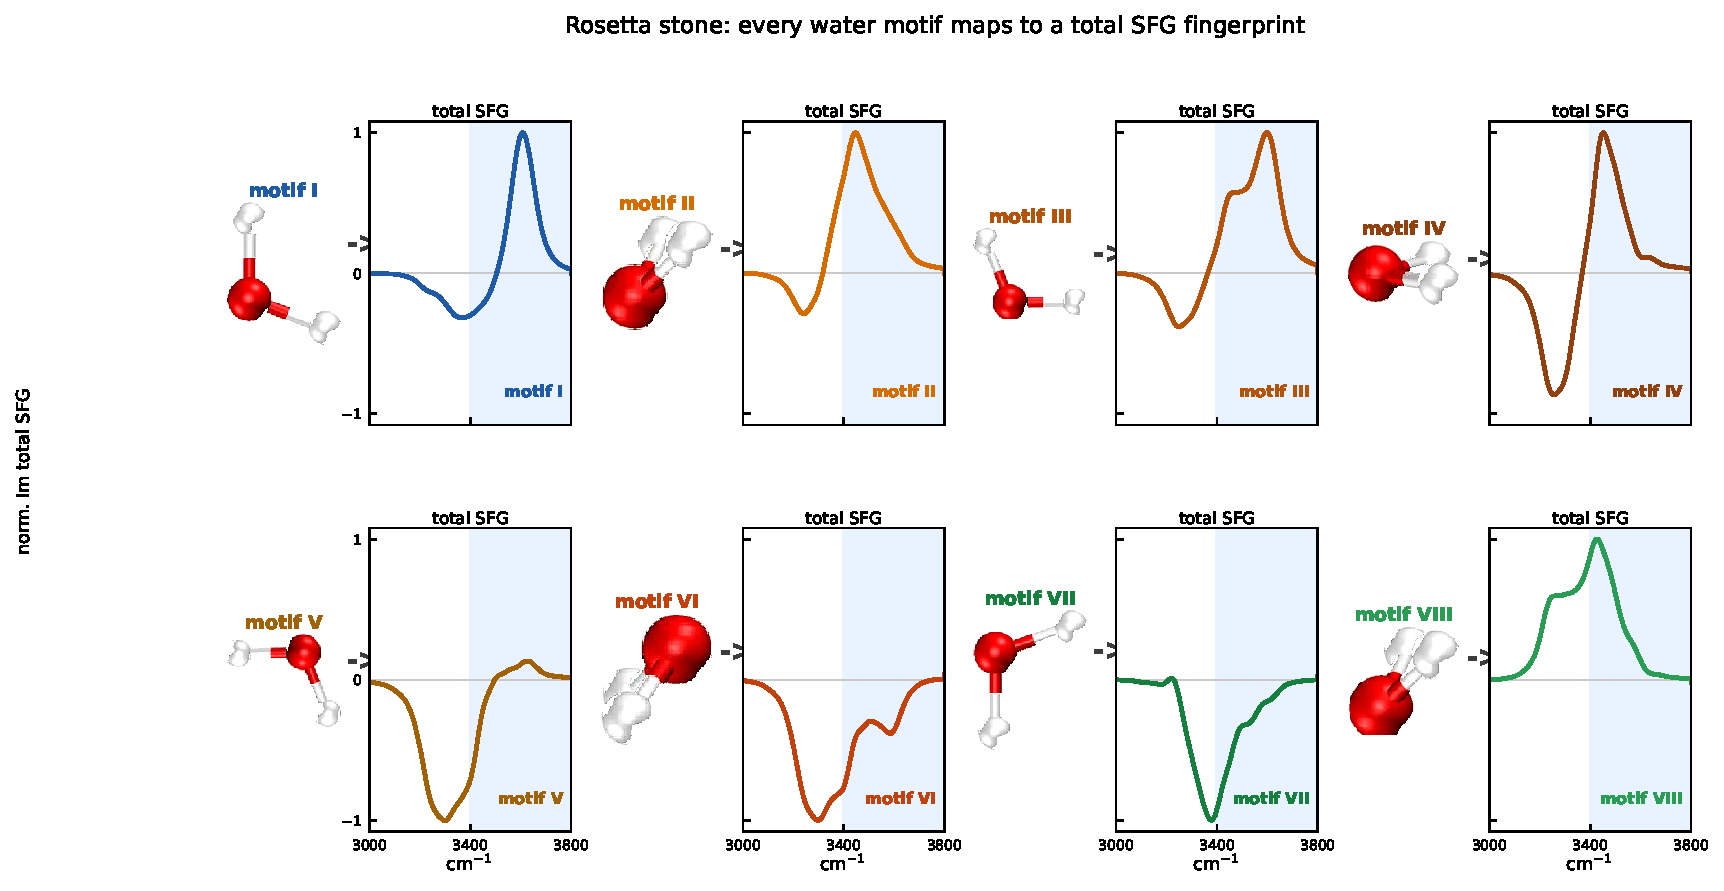
\includegraphics[width=\textwidth]{fig1_rosetta_pairs}
  \caption{One-to-one Rosetta-stone dictionary from the reference \waterair motif analysis, where every water motif maps directly to a total \sfg fingerprint. The structures are paired with their digitized total imaginary \sfg fingerprints from the corresponding total-SFG panels. Fingerprint amplitudes are normalized to their maximum absolute value for visual clarity. The silica/water analysis selects from this structural-to-spectral dictionary rather than fitting anonymous resonances.}
  \label{fig:rosetta-pairs}
\end{figure*}

For the buried-interface transfer, we relabel the selected depth sequence simply as L1--L3. These labels define an ordered water motif sequence rather than metric slabs: the layer order is inherited from the instantaneous interfacial definition of the \waterair analysis and is not converted into arbitrary fixed-thickness slices. The transfer also requires a sign convention. Because the silica/water spectrum was measured through the silica side, the paper-up direction of the \waterair structures is mapped toward silica. Positive \imchi is therefore interpreted as OH/H orientation toward the \ce{SiO2} side. Figure~\ref{fig:rosetta-selected} shows the three motifs selected for the primary model in this transferred geometry.

\begin{figure*}
  \centering
  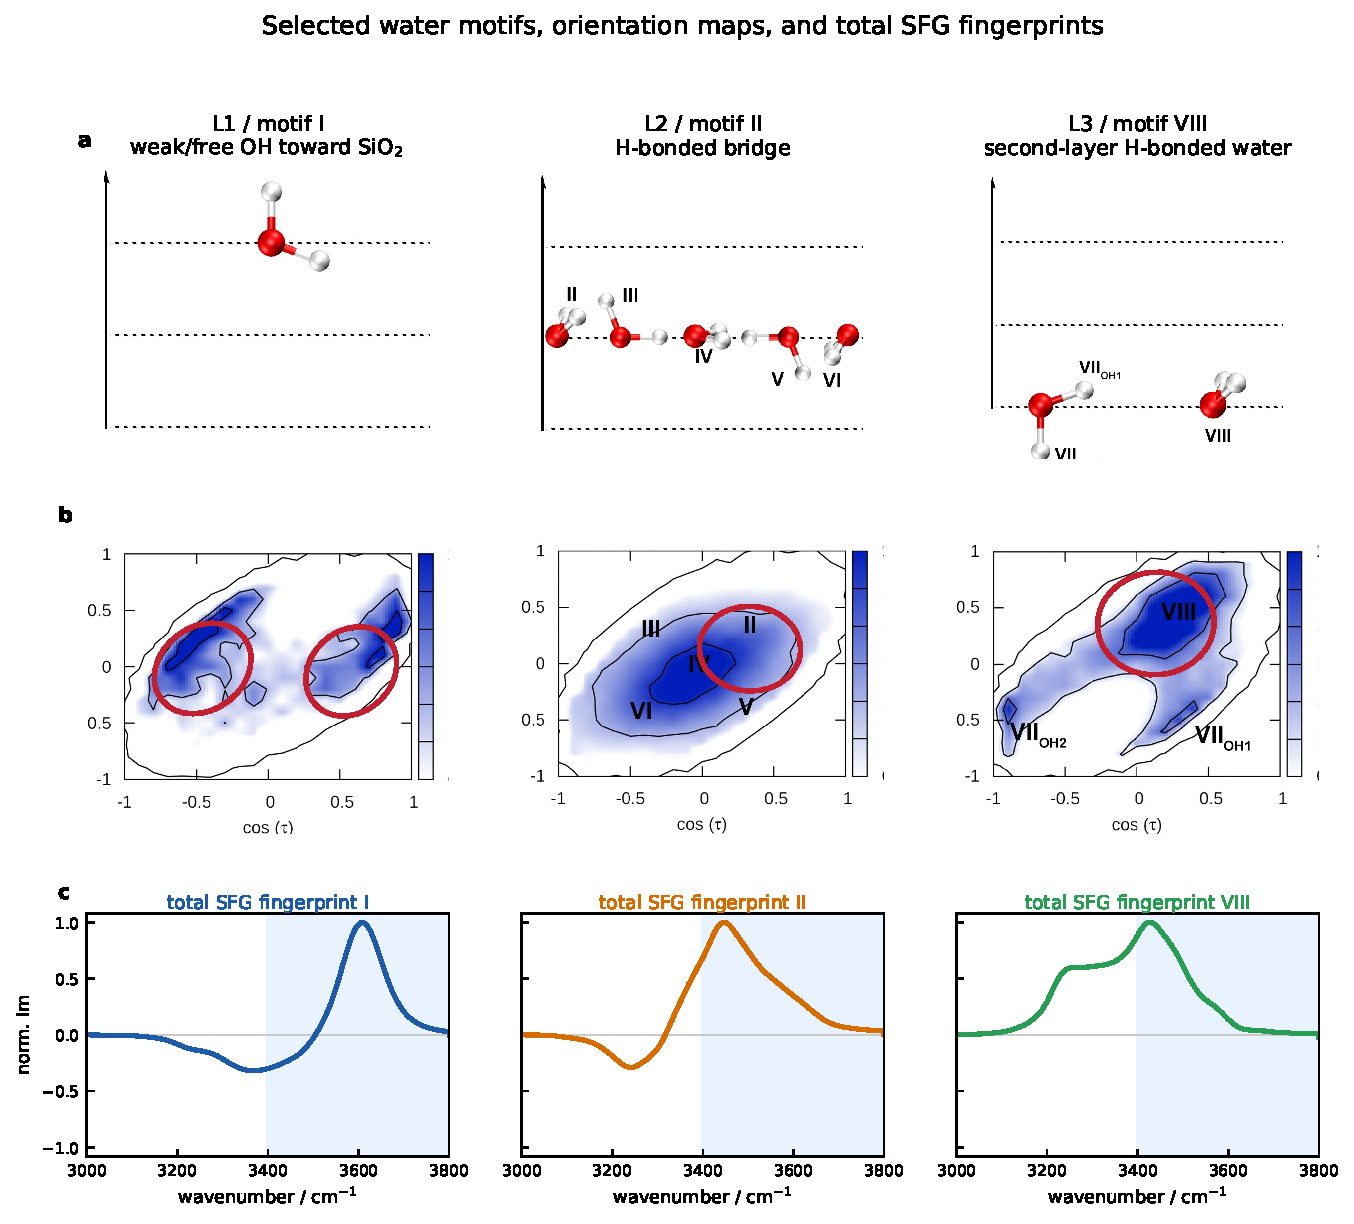
\includegraphics[width=\textwidth]{fig1_layer_rosetta}
  \caption{Rosetta-stone motif context for the silica/water model. (a) The complete water-motif fields from the reference analysis are shown by transferred depth: L1 contains motif I, L2 contains motifs II--VI, and L3 contains motifs VII and VIII. (b) The corresponding $\cos(\tau)$--$\cos(\xi)$ orientation maps highlight the motifs selected by the primary fit, I, VI, and VIII. (c) Digitized total imaginary \sfg fingerprints used in the transfer. The shaded region marks the primary physically interpretable \SIrange{3300}{3800}{cm^{-1}} OH-transfer window used for the experimental trace.}
  \label{fig:rosetta-selected}
\end{figure*}

\section{Experimental Trace and Structural Fit}

The experimental trace is supplied with the original frequency axis. The file contains one response channel rather than a full complex Re/Im pair. Consequently, the structural assignment is performed directly on the experimental trace. The raw trace contains nonfinite values only below the water OH-stretch region and is finite throughout the region used here. The analyzed window is defined from data-internal diagnostics: below \SI{3200}{cm^{-1}} the trace is outside the interpretable OH-transfer region, while \SIrange{3200}{3300}{cm^{-1}} displays a large raw-minus-smoothed fluctuation relative to its local amplitude. The primary physically interpretable OH-transfer window is therefore \SIrange{3300}{3800}{cm^{-1}}. This is not treated as the only valid spectral interval; broader low-edge and higher-frequency windows are used as diagnostic controls in the Supporting Information.

The fit uses digitized total \sfg fingerprints from the water--air Rosetta stone, a floating linear baseline, nonnegative motif weights, a global sign convention, and a global frequency shift. To reduce high-frequency point noise, the trace is smoothed by a 17-point moving average. This choice is not tuned to the final model: the I+VI+VIII assignment remains stable for smoothing windows from 7 to 33 points, with $R^2=0.9942$--0.9960 in the primary \SIrange{3300}{3800}{cm^{-1}} window and $R^2=0.9959$--0.9970 in the \SIrange{3400}{3800}{cm^{-1}} high-frequency control window. The window choice is also diagnostic rather than arbitrary. The \SIrange{3200}{3800}{cm^{-1}} interval is used as a broader diagnostic OH-window control, but it is more sensitive to the low-edge fluctuations. The \SIrange{3400}{3800}{cm^{-1}} window gives very high fits but removes the lower bonded-OH part that helps discriminate connector motifs. The \SIrange{3300}{3800}{cm^{-1}} window is therefore the best balance between data quality and structural information, selected from the measured trace and model-selection diagnostics rather than from a silica-specific structural prior.

\begin{figure*}
  \centering
  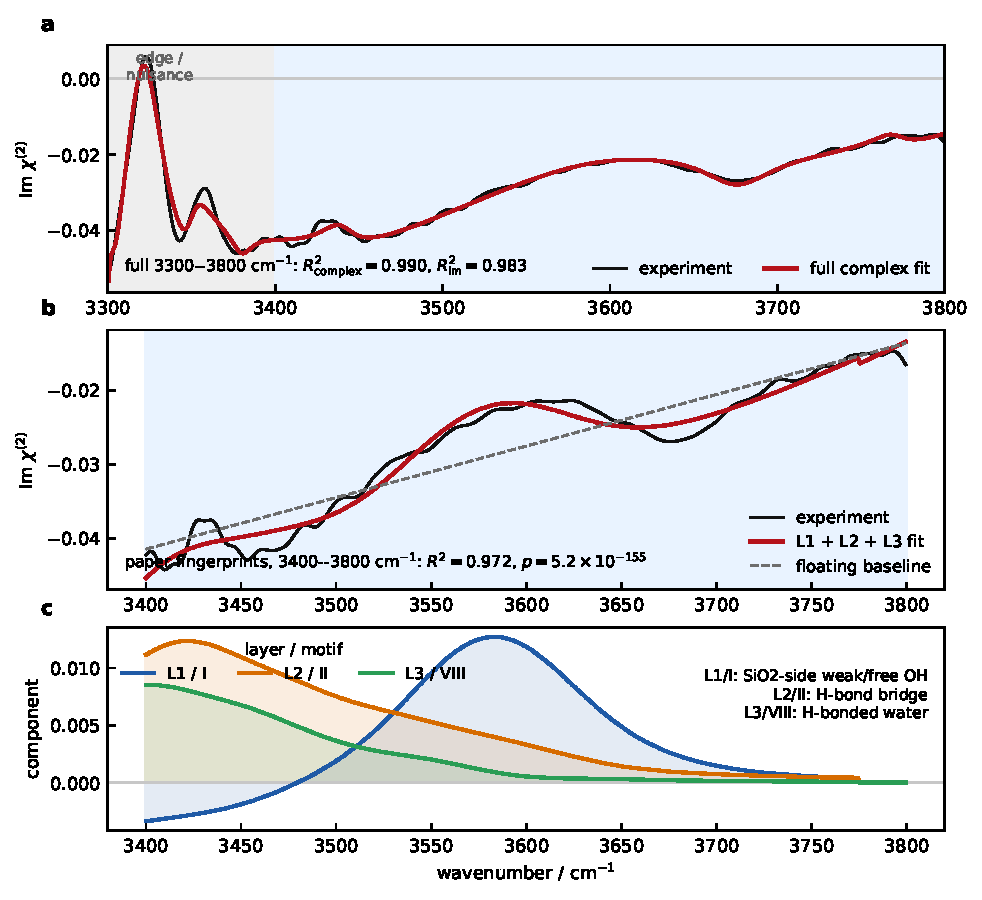
\includegraphics[width=0.88\textwidth]{fig2_sfg_fit}
  \caption{Structural fit to the silica/water experimental trace. (a) Raw and 17-point-smoothed experimental trace over the primary \SIrange{3300}{3800}{cm^{-1}} OH-transfer window. The lower-edge \SIrange{3300}{3400}{cm^{-1}} part of this window is shaded separately as a diagnostic region; the broader \SIrange{3200}{3800}{cm^{-1}} low-edge control is reported in the Supporting Information. (b) Nonnegative I+VI+VIII Rosetta-stone fit over \SIrange{3300}{3800}{cm^{-1}}, together with the nearly indistinguishable I+VI+VII+VIII control. The primary fit gives $R^2=0.9954$ with a global shift of \SI{+4}{cm^{-1}}. (c) Motif contributions to the primary fitted line shape. The weights are coherent, RMS-normalized SFG fingerprint weights, not molecule counts.}
  \label{fig:fit}
\end{figure*}

The primary three-motif I+VI+VIII model reproduces the experimental response with $R^2=0.9954$, an SSE of 0.0192, and $p<10^{-300}$ relative to a floating linear-background model (Fig.~\ref{fig:fit}). The $p$ value is the F-test probability for obtaining an equal or larger residual reduction when the motif fingerprints are added to the linear-background null model. It therefore quantifies spectral improvement against that null model. It is not the probability that a structural decomposition is unique, because neighboring smoothed points are correlated and the global frequency shift is reoptimized.

Several alternative models give similar high numerical quality, as expected for a one-dimensional coherent spectrum. A four-motif I+VI+VII+VIII control gives $R^2=0.9954$ with a slightly lower SSE, but the improvement is marginal and dominated by a small VII admixture. A direct I+VI+VII substitution for VIII fits much worse in the primary OH-transfer window ($R^2=0.9457$), whereas I+VI+VIII and I+VI+VII+VIII are visually indistinguishable. Thus, the dominant L3 response is assigned to motif VIII, while motif VII remains a symmetry-related/near-degenerate admixture that cannot be uniquely excluded from the one-dimensional SFG trace. A VI+VIII model without motif I reaches $R^2=0.9950$, showing that motif I is a small but resolved high-frequency marker rather than the dominant spectral contribution. Among the tested layered motif assignments, the data support a VI-type connector between the weak/free-OH marker and the dominant deeper bonded-water response.

\section{Layered Water Model}

The resulting water-only model is shown in Fig.~\ref{fig:model}. L1 is motif-I-like: one OH points toward silica and supplies the weak/free-OH marker, while the partner OH remains connected to the water network. L2 is motif-VI-like, a bridge-family connector that links the silica-side water to the deeper hydrogen-bonded layer. L3 is assigned primarily to motif VIII and dominates the coherent bonded-water response, with motif VII treated as a possible near-degenerate admixture rather than a uniquely excluded alternative. The RMS fingerprint fractions in the primary fit are 0.023 (I), 0.195 (VI), and 0.782 (VIII). These fractions should be read as spectral weights, not molecular populations, because \sfg amplitudes depend on orientation, vibrational coupling, and coherent interference.

\begin{figure*}
  \centering
  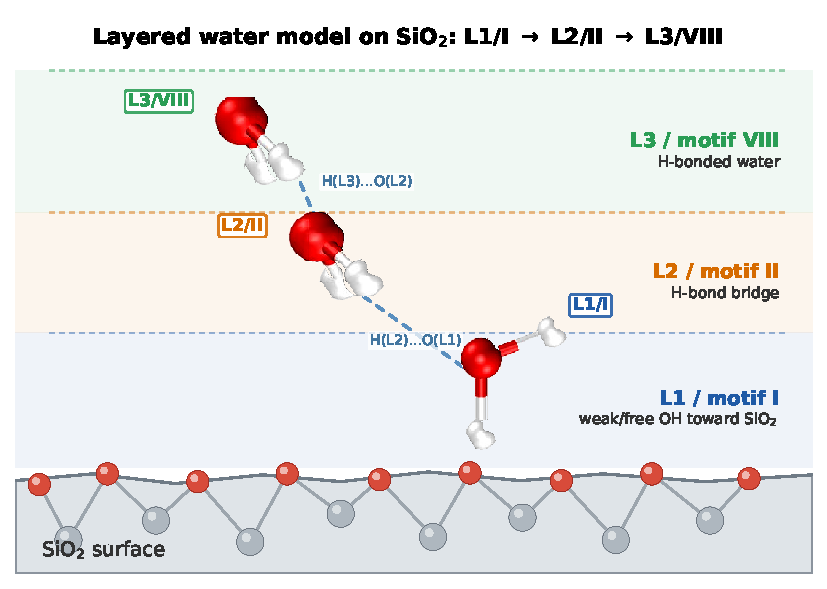
\includegraphics[width=0.95\textwidth]{fig3_layer_model}
  \caption{Three-motif layered water model on \ce{SiO2}. The dominant model is L1/I $\rightarrow$ L2/VI $\rightarrow$ L3/VIII. The silica slab is drawn above the water motifs so that the paper-up direction remains the silica-side direction. Colored arrows sketch the silica-side IR, visible, and SFG beam geometry. Dashed lines indicate hydrogen-bond connectivity between the weak/free-OH layer, the VI connector, and the deeper VIII-like bonded-water layer.}
  \label{fig:model}
\end{figure*}

The structural interpretation follows directly from the spectral assignment. The spectrum favors a VI-type connector in the bridge-family layer. The weak/free-OH marker emerges as a small terminal contribution embedded in a much larger bonded-water response. Only after the spectral assignment is made do we relate it to the silica-specific interpretation of Cyran \textit{et al.}: the inferred weak-OH marker is consistent with local weak-OH character at siloxane-like sites while the surrounding water remains largely hydrogen-bonded and connected to the oxide surface.

The relation to the neat water--air interface is therefore specific rather than global. At water--air, the weak/free-OH motif points toward vapor and is part of an intrinsically rough top layer.\cite{Kuhne2011JPCL,Kessler2015JPCB,Ohto2019JPCL} At silica/water, the analogous weak-OH marker points toward a solid oxide boundary, while the bonded part of the spectrum is reorganized by surface sites, interfacial fields, and the silica-side optical convention. Thus the Rosetta stone is used as a local structure--spectrum dictionary. It does not assert that the entire buried silica/water interface is water--air-like.

\section{Conclusions}

The silica/water spectrum can be reproduced with very high fidelity by nonnegative combinations of structure-resolved water--air total-\sfg fingerprints. The dominant model is a three-motif I+VI+VIII hydrogen-bonded water network: a small silica-facing weak/free-OH motif, a VI-type connector, and a dominant deeper response assigned to motif VIII. Motif VII remains a symmetry-related/near-degenerate admixture that cannot be uniquely excluded from the one-dimensional SFG trace, but it is not required for the main structural picture.

The result recovers the central conclusion of Cyran \textit{et al.} a posteriori: the high-frequency silica/water feature is consistent with a weakly hydrogen-bonded OH group oriented toward siloxane-like environments.\cite{Cyran2019PNAS} The added value of the Rosetta-stone analysis is that this marker is not assumed beforehand, but emerges from the transferred fingerprint basis and is then placed into a layer-resolved, hydrogen-bond-continuous water network. More generally, once the viewing geometry, sign convention, and data-supported water-fingerprint window are defined, phase-resolved \sfg spectra can be interpreted by molecularly assigned total-\sfg responses rather than by anonymous resonances alone.

\section{Methods}

The experimental trace was read from \path{heat2_fud.txt} with the corresponding frequency axis in \path{xaxis_fud.txt}. Nonfinite values occur only below the water OH-stretch window and were filled by interpolation for plotting continuity; all reported structural fits use finite data in the selected OH-stretch windows. The primary physically interpretable OH-transfer fit uses the \SIrange{3300}{3800}{cm^{-1}} region selected from raw-minus-smoothed trace diagnostics and model-discrimination tests. The trace is smoothed by a 17-point moving average for the primary analysis. Smoothing windows from 7 to 33 points were tested as controls.

Species-resolved total \imchi fingerprints were digitized from the \waterair motif analysis.\cite{Kaliannan2026Rosetta} Each fingerprint was interpolated onto the experimental frequency grid, shifted over a discrete frequency grid, multiplied by a global sign convention, and combined with nonnegative least squares plus a floating linear baseline. The primary fit allowed a conservative global shift range of \SI{\pm20}{cm^{-1}}. Reported $p$ values are F-test diagnostics for residual reduction relative to a linear-background model. They are used as measures of spectral improvement, not as exact probabilities assigned to a unique molecular structure.

\section*{Supplementary Material}

The Supporting Information contains the processed experimental trace, primary I+VI+VIII fit curve, RMS-normalized weights, smoothing/window sensitivity table, exact motif-candidate comparison, window-choice diagnostics, and direct VII/VIII L3-control fits.

\section*{Acknowledgments}

Part of this research was funded by the Deutsche Forschungsgemeinschaft (DFG, German Research Foundation) through project numbers 417590517/CRC1415 and 519869949.

\section*{Author Declarations}

\subsection*{Conflict of Interest}

The authors have no conflicts to disclose.

\subsection*{Author Contributions}

Jen{\'e}e D. Cyran: experimental data, conceptual framing, methodology, interpretation, visualization, and writing--review and editing. Thomas D. K{\"u}hne: conceptualization, investigation, methodology, software, formal analysis, visualization, and writing--original draft.

\section*{Data Availability}

The digitized spectra, transferred fingerprints, fitting scripts, processed output tables, raw experimental trace, and figure-generation code are available in the public GitHub repository \url{https://github.com/DCM-Uni-Paderborn/sio2-water-sfg-rosetta}.

\bibliographystyle{aipnum4-2}
\bibliography{references}

\end{document}
